
\subsection{Exkurs Umformtechnik}


Da die Gegenstände und Verfahren dieser Untersuchung in das Gebiet der Umformtechnik fallen, werden die ausschlaggebendsten Begriffe und Sachverhalte dieses komplexen Gebietes noch einmal vereinfacht und komprimiert umrissen. So ist es möglich über ein theoretisches Gerüst zu verfügen welches später behilflich sein wird   Analogien zu den durchzuführenden Prozessen zu erkennen.
\subsubsection{Systematisierung Formgebungsverfahren}
Umformverfahren können
auf Grund der unterschiedlichen Spannungsverhältnisse in fünf verschiedene Gruppen unterteilt werden. Einfache Beschreibungen der Spannungsverhältnisse sind kaum möglich denn,  abhängig von der Art der Operation, können  unterschiedliche Spannungen gleichzeitig auftreten oder sich sogar  während des Formgebungsvorgangs verändern. Deshalb werden die überwiegenden Spannungen als Klassifikationskriterium ausgewählt. Folgende fünf Gruppen der Umformprozesse werden definiert:
\begin{enumerate}
\item \emph{Druckumformen} nach DIN 8583 behandelt die Formgebung eines festen Körpers  welche den  plastifizierten  Zustand hauptsächlich durch uni- oder multiaxiale Druckbelastungen herbeiführt.
\item \emph{Zugdruckumformen} nach DIN 8584 behandelt die Formgebung eines festen Körpers  welche den plastifizierten Zustand  hauptsächlich durch kombinierte uni- oder multiaxiale Zug- und Druckbelastungen herbeiführt.
\item \emph{Zugumformen} nach DIN 8585 behandelt die Formgebung eines festen Körpers welche den plastifizierten Zustand überwiegend durch uni- oder multiaxiale Zugbelastungen verursacht.
\item \emph{Biegeumformen} nach DIN 8586 behandelt die Formgebung eines festen Körpers welche den plastifizierten Zustand hauptsächlich durch eine Biegebelastung herbeiführt.
\item \emph{Schubumformen} nach DIN 8587 behandelt die Formgebung eines festen Körpers welche den plastifizierten Zustand überwiegend durch eine Schubbelastung herbeiführt.

\end{enumerate}

Von untergeordneter Bedeutung sind innerhalb dieser Gruppen  weitere Unterteilungen auf der Grundlage von kinematischen Überlegungen (z.B. Relativbewegung zwischen Werkzeug und Werkstück), Werkzeug- und Werkstück Geometrien sowie Beziehungen zwischen den beiden möglich. Die Klassifizierung formgebender Methoden unterlässt bewusst die Frage ob ein Prozess durch Erwärmung, bei Raumtemperatur oder weiterer Wärmebehandlung stattfindet. Früher  wurde zur Abgrenzung zwischen Kalt- und Warmformen die Rekristallisationstemperatur gewählt. Obwohl diese sicherlich das Verhalten  von Werkstückmaterialien während der Formgebung beeinflusst, zählt heutzutage zur Allgemeinerkenntnis das die spontane Erholung  eine weitaus größere Rolle in schnellen Umformprozessen spielt. Außerdem führt die herkömmliche Terminologie angesichts der großen Vielfalt  an Materialien die verwendet werden leicht zu Missverständnissen. So würde zum Beispiel die Formgebung von Blei bei Raumtemperatur als \emph{Warmumformen} deklariert während Molybdän bei einer Temperatur von 800 Grad Celsius noch als \emph{Kaltumformen} eingestuft wäre. Aus diesem Grunde unterscheidet DIN 8582 zwischen Formgebung bei Raumtemperatur und Formgebung bei einem auf über Raumtemperatur erwärmten Werkstücks. Überdies ist zu Berücksichtigen ob ein permanenter Temperaturwechsel während des Umformvorgangs stattfindet. Mit Hilfe dieser beiden Kriterien ist eine weiter Unterteilung von den Metall Umformverfahren möglich:

\begin{enumerate}
\item Formgebung nach Erwärmung (Warmumformen)
\item Formgebung ohne Erwärmung (Kaltumformen)
\end{enumerate}

Beide Punkte können weiter eingestuft werden in:

\begin{itemize}
\item Formgebung ohne Veränderung der mechanischen Eigenschaften
\item Formgebung mit temporärer Veränderung der mechanischen Eigenschaften
\item Formgebung mit permanenter Veränderung der mechanischen Eigenschaften
\end{itemize}

In der Industriepraxis kommen letztendlich unzählige Kombinationen der oben aufgeführten Unterteilungen vor.\footcite[Vgl.][2.1ff]{kl}
\subsubsection{Metallurgische Zusammenhänge}
In diesem Abschnitt wird erörtert was auf makroskopischer und mikroskopischer Ebene in metallischen Werkstoffen bei Formänderungsprozessen vor sich geht. Überdies soll ein Einblick gewonnen werden wie sich die verschiedenen Einflussgrößen während eines Umformvorgangs gegenseitig beeinflussen.
\su{Kristallaufbau}
In der Umformtechnik werden zum Großteil metallische Bauteile erzeugt. Eisen- wie Nichteisenmetalle bestehen aus metallisch gebundenen Atomen. Sie bekommen ihren Zusammenhalt aus einer sie gleichmäßig umgebenden frei beweglichen Elektronengaswolke, die aus abgegebenen Valenzelektronen besteht und so die positiven Metallionen  durch die sogenannte \emph{Metallbindung} bindet.\footcite[Vgl.][12]{wki} Ihr wichtigstes Merkmal ist der kristalline Aufbau. Darunter versteht man die feste, regelmäßige Struktur der Atome. In der Physik sowie in der Chemie existieren verschiedene Modelle über den Aufbau und das Aussehen solcher Kristallgebilde. In \fref{fig:makromikro}\footcite[Vgl.][4]{fu} wird eine Elementarzelle des $\alpha $-Eisen unter mikroskopischen (atomistischen) und makroskopischen Gesichtspunkten dargestellt. Oben rechts im Bild sind die drei Elementarzellen abgebildet aus denen Metalle zusammengesetzt sind. Es handelt sich um die  kubisch-raumzentrierte , kubisch-flächenzentrierte und hexagonale (das hdP steht für hexagonal dichteste Packung) Elementarzellen.\footcite[Vgl.][3-5]{fu}
\begin{figure}
\centering
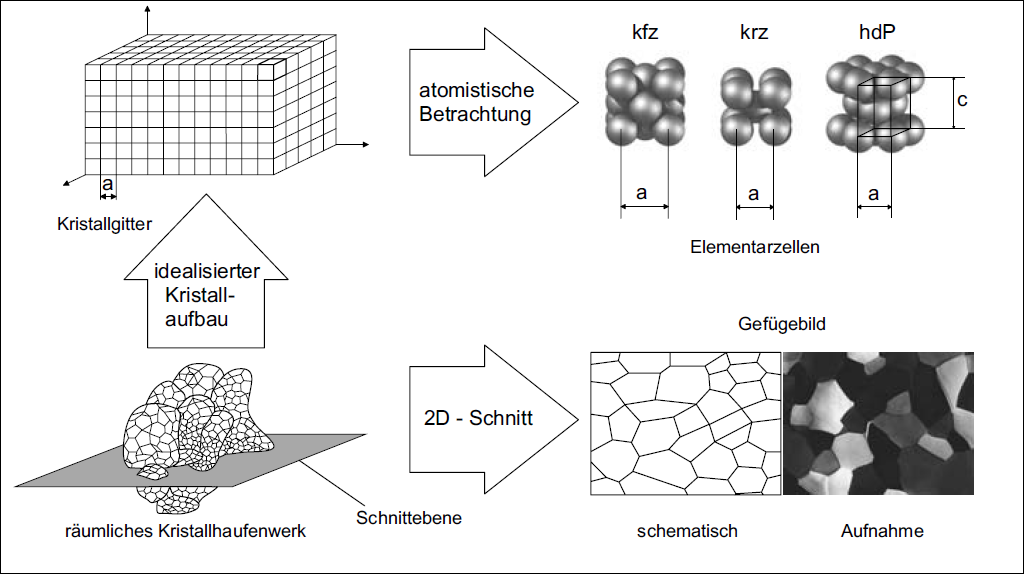
\includegraphics[width=0.8\textwidth]{makromikro}
\caption{Aufbau eines Kristallgitter mikroskopisch (atomistisch) und makroskopisch.}
\label{fig:makromikro}
\end{figure}
Das kleinste Kristall im Metallgitterverband ist das sogenannte \emph{Einkristall} (siehe \fref{fig:elementarzellen})\footcite[Vgl.][37]{hu} es besitzt folgende Merkmale\begin{itemize}
\item allseitig freie Oberfläche
\item keine Korngrenzen
\item Fehlstellen wie z.B. Leerstellen, Versetzungen
\item anisotropisches Verhalten wegen bevorzugter Gleitrichtungen. Unter \emph{Anisotropie} wird das Auftreten von unterschiedlichen mechanischen und physikalischen Eigenschaften in die verschiedenen Raumrichtungen verstanden (z.B. Sperrholz). Im Gegensatz dazu weist \emph{isotropisches} Verhalten gleiche mechanische und physikalische Eigenschaften in die verschiedenen Raumrichtungen auf (z.B. Sonnenlicht)\footcite[vgl.][37]{hu}
\begin{figure}
\centering
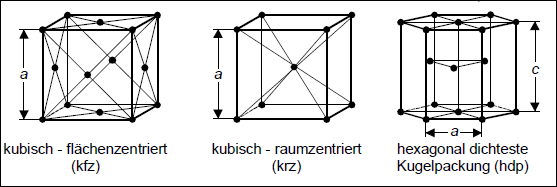
\includegraphics[width=0.8\textwidth]{elementarzellen}
\caption{Elementarzellen (Einkristalle)}
\label{fig:elementarzellen}
\end{figure}

\end{itemize}
Die kleinste geometrisch zusammenhängende Einheit eines Kristallgitters ist die Elementarzelle. Knüpft man hypothetisch, in Richtung aller drei Koordinatenrichtungen, Elementarzellen aneinander entsteht ein Kristallgitter (siehe \fref{fig:makromikro} oben links). Das geometrische Aneinanderreihen von Elementarzellen erzeugt \emph{Idealkristalle} (fehlerfreie Kristalle) die so in der Realität nicht vorhanden sind. In der Realität sind in einem Raumgitter der Metalle zahlreiche Gitterfehler vorhanden. Hier wird unterschieden in folgende signifikante Gitterfehler:
\begin{enumerate}
\item  \emph{Nulldimensionale Gitterfehler} (punktförmig):\begin{itemize}
\item \emph{Zwischengitteratome} liegen vor wenn Atome auf Zwischengitterplätzen angeordnet sind. 
\item \emph{Austausch- oder Substitutionsatome}. Die Atomplätze werden von Fremdatomen beansprucht.
\item \emph{Einlagerungsatome} entstehen wenn die Zwischengitterplätze von Fremdatomen vereinnahmt werden.
\item \emph{Leerstellen} treten auf wenn wenn einzelne Gitterplätze nicht von Atomen besetzt werden. Sie sind bedeutend bei thermisch aktivierten Diffusionsvorgängen.
\end{itemize}
\item \emph{Eindimensionale Gitterfehler} sind linienförmige Strukturfehler (Versetzungen)(siehe \fref{fig:versetzung})\footcite[Vgl.][50]{wk}.

\begin{figure}
\centering
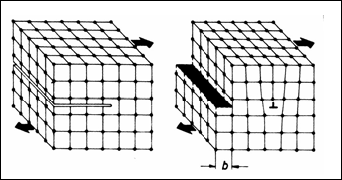
\includegraphics[width=0.8\textwidth]{versetzung}
\caption{Stufenversetzung}
\label{fig:versetzung}
\end{figure}
 Diese sind für Umformprozesse von übergeordneter Bedeutung weil sie die plastische Formgebung besonders beeinflussen.
\item \emph{Zweidimensionale Gitterfehler} entstehen bei Oberflächendefekten. Die wichtigsten sind Korngrenzen und Phasengrenzflächen. Wenn ein Metall aus dem flüssigen Zustand kristallisiert wachsen die Keime zuerst an verschiedenen Stellen unabhängig voneinander. Im Laufe des Abkühlungsprozesses wachsen die Keim aufeinander zu und bilden Korngrenzen.
\end{enumerate}

Der Unterschied zwischen Real- und Idealkristallen ist in diesen Gitterfehlern begründet. Die Zugfestigkeit des Eisens liegt  z.B mehr als zwei Zehnerpotenzen unter der theoretisch Möglichen im Fall des Vorhandenseins eines Idealkristalls. Die Abstände der Atome sind in den Elementarzellen in verschiedene Richtungen unterschiedlich ausgeprägt. Das ist die Ursache für die Richtungsabhängigkeit bestimmter Eigenschaften der Metalle. Bestimmte Herstellungsverfahren (z.B. einige Walzverfahren, gerichtete Erstarrung) zielen darauf ab die Orientierung der Kristallite in eine bestimmte Richtung zu beeinflussen. Dieses Vorgehen bezeichnet man als Textur. Sie ermöglicht das die Werkstoffeigenschaften richtungsabhängig werden.  Die Richtungsabhängigkeit wird wie schon oben erwähnt mit dem Begriff der \emph{Anisotropie}. 
Während des Erstarrungsprozesses technischer Schmelzen werden Verunreinigungen überwiegend vor der Erstarrungsfront hergeschoben. Es bilden sich Ansammlungen von Verunreinigungen an den Korngrenzen. Ein reales Gefüge ist durch einen metallogfrafischen Schliff im Lichtmikroskop zu erkennen und mit einem schematischem Gefüge verglichen (siehe \fref{fig:makromikro}) . Es sind lediglich Größe, Anordnung und Form der Kristalle erkennbar zu machen. Die innere Struktur ist nicht sichtbar zu machen.\footcite[Vgl.][3-6]{fu}

\subsubsection{Verformung Prinzipiell}
Die Duktilität (plastische Verformbarkeit) der Metalle ist eine Eigenschaft welche in der Umformtechnik die größte Bedeutung hat. Hier ist es sinnvoll die Vorgänge wieder an einem Idealkristall (besitzt keine Gitterfehler) darzustellen. Bei geringen Belastungen tritt im Bauteil keine bleibende Verformung ein, es geht nach  der Entlastung wieder in seinen Ausgangzustand zurück. Man nennt dies \emph{elastische} Verformung. Bei der \emph{plastischen} Verformung gleiten Kugelschichten im Gitterverband aneinander vorbei,  nach Entlastung kehrt das Bauteil nicht mehr in seine ursprüngliche geometrische Form zurück (siehe \fref{fig:eloplastkristall})\footcite[Vgl.][45]{wk}.
\begin{figure}
\centering
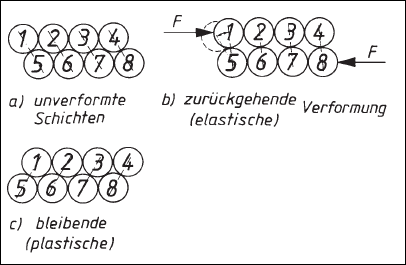
\includegraphics[width=0.8\textwidth]{eloplastkristall}
\caption{Verformung elastisch und plastisch}
\label{fig:eloplastkristall} 
\end{figure}
Das die plastische Verformung begünstigende Gleiten findet in den sogenannten \emph{Gleitebenen} statt. Diese befinden sich zwischen den Atomschichten mit der größten \emph{Packungsdichte}. Aufgrund dieser höheren Packungsdichte ist der Abstand der einzelnen Schichten nicht so groß und dem Verschieben der Schicht wird dort der  geringste Widerstand entgegengesetzt. Im Gegensatz zum Idealkristall sind aufgrund von Versetzungen die kritischen Schubspannungen, welche zur plastischen Verformung benötigt werden,  erheblich kleiner. Bei dem Idealkristall stellen wir uns ein schrittweises Gleiten ganzer Atomschichten vor während bei Realkristallen ein schrittweises Wandern der Atomreihen entlang der Versetzungslinien stattfindet. Man kann dies auch mit dem Wandern einer Teppichfalte vergleichen (siehe \fref{fig:wandernstufenversetzung}) \footcite[Vgl.][53]{wk}. Wenn z.B. ein sehr langer schwerer Teppich eine Falte hat erfordert es hohe Kräfte um durch Zug an einem Teppichende die Falte zu glätten. Wesentlich geringer ist der Kraftaufwand wenn man die Falte direkt langsam aus dem Teppich kämmt.\footcite[Vgl.][45-53]{wk}
\begin{figure}
\centering
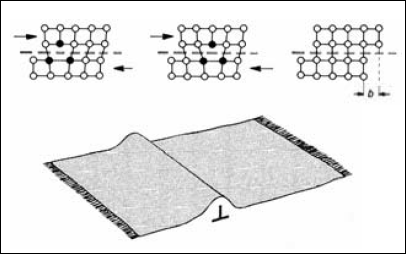
\includegraphics[width=0.8\textwidth]{wandernstufenversetzung}
\caption{Wandern einer Stufenversetzung in Analogie zum Wandern einer Teppichfalte}
\label{fig:wandernstufenversetzung}
\end{figure}

\subsubsection{Rekristallisation, Erhohlung und Kaltverfestigung}
Ein wichtiger Faktor bei der Formänderung in metallischen Werkstoffen ist die Umformtemperatur und die thermisch aktivierten Vorgänge die diese eventuell im atomaren Gitterverband des Werkstoffes auslösen. Während eines Umformvorgangs erhöht sich stufenweise der Energiegehalt des Werkstoffmaterials. Dies ist größtenteils durch Versetzungen und plastische Verzerrungen im Gitterverband bedingt. Die Versetzungsdichte steigert sich direkt proportional zu dem Umformgrad. Man nennt dies \emph{Kaltverfestigung}. Bei fortgeschrittenem Umformgrad gerät durch den erhöhten Energieaufwand Wärme in das Material was bewirkt, dass sich die Atome wieder dem Gleichgewichtszustand annähern wollen. Ab einem bestimmten Überschreiten des kritischen Umformgrades speichert sich innere Energie im Gitterverband und kann so eine \emph{Erhohlung} der Gitterfehler und Rückbildung der Versetzungen bewirken. Bei noch höherer Energiezufuhr kann es sogar zur \emph{Rekristallisation} (Bildung von Subkorngrenzen und erneutem Kornwachstum kommen, was ein neues entspanntes und duktiles Gefüge mit sich bringt (siehe \fref{fig:rekristall})\footcite[Vgl.][13]{fu}.\footcite[Vgl.][11-13]{fu}
\begin{figure}
\centering
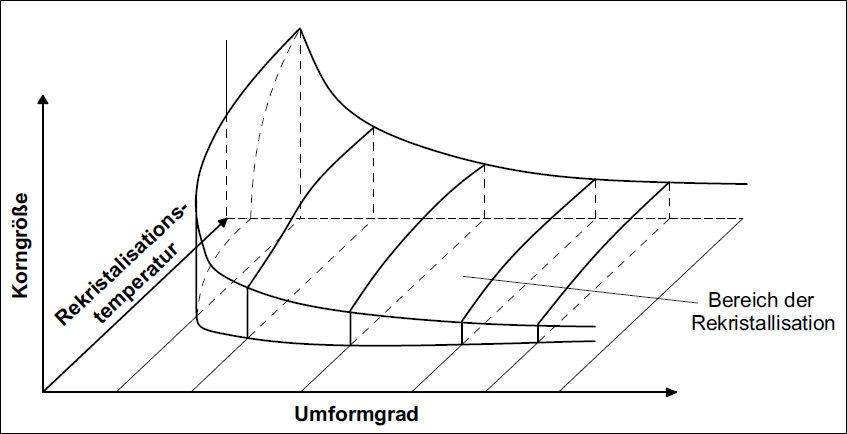
\includegraphics[width=0.8\textwidth]{rekristall}
\caption{Zusammenhang Umformparameter und Rekristallisation}
\label{fig:rekristall}
\end{figure}





\subsubsection{Eigenspannungen}
Das Thema Eigenspannungen im Zusammenhang mit der Verarbeitung von Blechen an die hohe Qualitätsanforderungen gestellt werden ist natürlich von besonderem Interesse bei der Analyse von Problemstellungen die auf den einzelnen Fertigungsstufen entstehen können. Es handelt sich dabei um Spannungen in einem sich im Temperaturgleichgewicht befindenden Bauteil, auf das keine mechanischen Beanspruchungen wirken. Die mit den Eigenspannungen involvierten  Beanspruchungen stehen im mechanischen Gleichgewicht zueinander. Bei Bauteilen und Werkstücken die unter Eigenspannung stehen kann ein Materialversagen wesentlich schneller eintreten da sich die tatsächlich wirkende Spannung aus Eigenspannungen und Spannungen von außen einwirkenden Kräften zusammensetzt. Durch die Eigenspannungen kann auf Grund des daraus resultierenden gestörten Gleichgewichtszustands plastische Formänderung in Form von Verzug auftreten.
Dabei wirken sich Druckeigenspannungen in der Bauteilrandzone meist vorteilhaft aus da sie einer möglichen Rissbildung und Rissausbreitung entgegenwirken.

Es wird im Hinblick auf Auswirkungen auf das Bauteilvolumen eine Unterteilung der Eigenspannungen in drei Gruppen unternommen:
\begin{enumerate}
\item \emph{Makroskopische Eigenspannungen}, welche sich homogen über mehrere Kristallite erstrecken. Bei Störung des Gleichgewichts führen sie zu makroskopischen Formänderungen.
\item \emph{Eigenspannungen}, die in kleinen Abschnitten homogen sind und bei Störungen des Gleichgewichts zu makroskopischen Formänderungen führen.
\item \emph{Mikroskopische Eigenspannungen}, welche durch inhomogene Versetzungsreihen ausgelöst werden und über wenige Atombereiche variieren. Sie tragen nicht zu makroskopischen Formänderungen bei. 


\end{enumerate}

Eigenspannungen werden verursacht durch inhomogene Deformationen im Bauteil, was zu einer weiteren Einteilung führt.

Entstehungsursachen sind:
\begin{itemize}
\item \emph{Thermische Eigenspannungen} (siehe \fref{fig:eigenspanabk})\footcite[34]{hu} die bei Abkühlung eines Bauteils entstehen.\begin{figure}
  \centering
  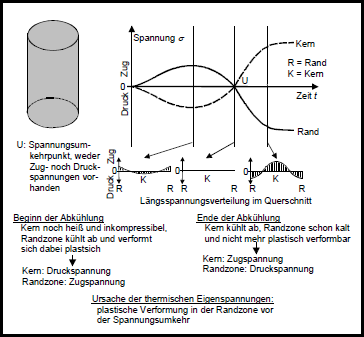
\includegraphics[width=0.8\textwidth] {eigenspanabk}
  \caption{Zeitliche Änderung der Längsspannungsverteilung im Querschnitt eines Zylinders bei schneller Abkühlung.}
  \label{fig:eigenspanabk}
  \end{figure}

\item \emph{Verformungseigenspannungen} (siehe \fref{fig:eigenspanfaser} und \fref{fig:eigenspandrahtzieh})\footcite[34]{hu} welche durch inhomogene Verformung auf Grund äußerer Beanspruchung verursacht werden.\begin{figure}
  \centering
  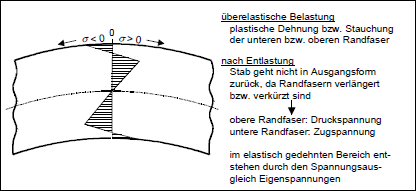
\includegraphics[width=0.8\textwidth]{eigenspanfaser}
  \caption{Schematische Längseigenspannungsverteilung im Querschnitt eines Stabs nach plastischer Biegebeanspruchung.}
  \label{fig:eigenspanfaser}
  \end{figure}
  \begin{figure}
  \centering
  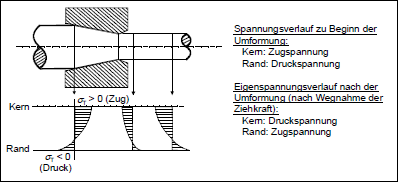
\includegraphics[width=0.8\textwidth]{eigenspandrahtzieh}
  \caption{Schematische Tangentialeigenspannungsverteilung beim Drahtziehen in Abhängigkeit von der Ziehdüsenentfernung.}
  \label{fig:eigenspandrahtzieh}
  \end{figure}
\item \emph{Umwandlungseigenspannungen} (siehe \fref{fig:eigenspanmol})\footcite[35]{hu} die durch inhomogene Gefügeumwandlungen  
mit einer einhergehenden Volumenänderung ausgelöst werden.\begin{figure}
  \centering
  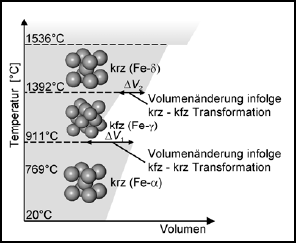
\includegraphics[width=0.8\textwidth]{eigenspanmol}
  \caption{Volumenänderung durch Veränderung der Gitterstruktur.}
  \label{fig:eigenspanmol}
  \end{figure}
\end{itemize}

Bei dem Messen von Eigenspannungen wird in zerstörende sowie zerstörungsfreie Erfassungsmethoden unterschieden. Hier wird hauptsächlich auf die zerstörenden Verfahren eingegangen und unter den zerstörungsfreien nur die Finite-Elemente-Methode kurz erläutert. Für zylindrische Bauteile werden Ausbohr- und Abdrehverfahren verwendet um die Eigenspannungen in radialer, tangentialer sowie axialer Richtung zu erfassen.Die Eigenspannungen in Platten und Stäben werden mit schichtweisem Abtragen, Einschneiden und Aufschlitzen ermittelt.\begin{figure}
  \centering
  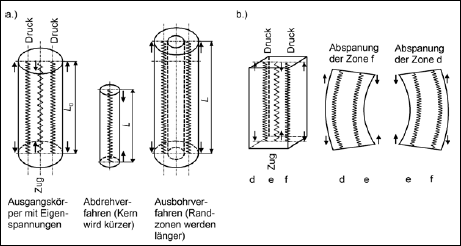
\includegraphics[width=0.8\textwidth]{eigenspanschnitt}
  \caption{Ermittlung von Eigenspannungen a) in zylindrischen Bauteilen und b) in Platten und Stäben.}
  \label{fig:eigenspanschnitt}
  \end{figure}
  Nach der jeweiligen Entfernung des Materials lassen sich Bauteilgeometrieänderungen sehr gut erkennen oder auch mit Messgeräten erfassen und daraus  sind Schlüsse auf die Art und Lage der spezifischen Eigenspannungen abzuleiten (siehe \fref{fig:eigenspanschnitt})\footcite[36]{hu}. Zur ganz präzisen Analyse  und Visualisierung von Bauteilspannungen kommt heutzutage in der Industrie  die FEM (Finite-Elemente-Methode zum Einsatz).\footcite[Vgl.][32-37]{hu} Mit ihr lassen sich Umformprozesse sehr gut simulieren. Die FEM ist ein numerisches Verfahren zur näherungsweisen Lösung kontinuierlicher Feldprobleme. Darunter versteht man Probleme, in denen das Verhalten des Kontinuums durch partielle, orts- und zeitabhängige Differentialgleichungen umschrieben wird. Für jede Zustandsgröße eines Kontinuums gehören unendlich viele Werte, weil sie eine Funktion jedes Punktes des Kontinuums beschreibt. Die FEM zerlegt das Kontinuum in \emph{endlich} viele Teile, die sogenannten \emph{finiten Elemente}. Ein komplexes, kontinuierliches Problem wird dabei in eine endliche Zahl einfacher, voneinander abhängiger Probleme unterteilt.\footcite[Vgl.][48]{fu}
\subsubsection{Umformgrad}
In der Umformtechnik wird zwischen elastischer und plastischer Formänderung unterschieden. Bildet sich ein Körper nach einer Deformation vollständig zu seiner ursprünglichen Geometrie zurück so ist er in dem elastischen Bereich gedehnt worden. Wird ein Bauteil über diesen Bereich hinaus gedehnt so tritt eine bleibende Verformung ein, was man unter plastifizierten Zustand versteht.  Bei herkömmlichen einachsigen Zug- oder Druckversuchen werden Spannung und Dehnung auf Ihre Ausgangsgrößen bezogen z.B. \begin{equation}\sigma=\frac{F}{A_o}\end{equation} oder für die Dehnung \begin{equation}\varepsilon = \frac{\Delta l}{l_0}\end{equation} Diese Methode der Festigkeitsberechnung ist für Bauteile die konstruktionsbedingt für den elastischen Bereich dimensioniert werden   durchaus ausreichend. In der Umformtechnik sind aber die \emph{wahren Spannungs- und Dehnungsverhältnisse} von großer Bedeutung. Die wahre Spannung, die die momentan einwirkende Kraft auf die momentane Fläche bezieht ist die \emph{Fließspannung} $ k_f $. Für die \emph{wahre Dehnung} die den eigentlichen Umformgrad $ \varphi $ darstellt bezieht sich auf den sich mit der Verformung ändernden Bezugswert. Eine Herleitung die z.B. bei einem einachsigen zylindrischen Druckversuch in dem der Höhenunterschied \begin{equation}
h=h_1-h_0 \end{equation}  den zurückgelegten Stempelweg darstellt ist:\begin{equation}
\varphi=\int\limits_{h_0}^{h_1}\frac{dh}{h}=\ln h_1 - \ln h_0 = \ln\frac{h_1}{h_0}\end{equation} Im Falle des Druckversuchs ergibt sich dafür natürlich ein negativer Umformgrad. Erwähnt werden sollte in diesem Zusammenhang noch das Gesetz der \emph{Volumenkonstanz} welches aussagt das  bei plastischen Fließvorgängen das Volumen des Kontinuums unverändert bleibt. So kann man den Stauchvorgang eines Vierkantstabes so beschreiben: 






 \begin{equation}h_1 \cdot  b_1 \cdot l_1 = h_0 \cdot b_0 \cdot l_0\end{equation} 
Nach Transformation und Logarithmieren der Gleichung erhält man
das Gesetz der Volumenkonstanz. 
 
 
 \begin{equation}\ln (\frac{h_1}{h_0} \cdot \frac{b_1}{b_0} \cdot \frac{l_1}{l_0}) = \ln 1 = 0\end{equation} 
 
daraus folgt \begin{equation}
\ln\frac{h_1}{h_0}+\ln\frac{b_1}{b_0}+\ln\frac{l_1}{l_0}=\varphi_1+\varphi_2+\varphi_3=0
\end{equation}
Analog dazu gilt für die Umformgeschwindigkeiten
\begin{equation}
\dot{\varphi_1}+\dot{\varphi_2}+\dot{\varphi_3}=0
\end{equation}

Durch den hydrostatischen Spannungsanteil beschriebene Dehnungen und Dehngeschwindigkeiten werden bei plastischen Fließvorgängen gleich null.\footcite[Vgl.][24-28]{fu}
\subsubsection{Umformgeschwindigkeit}
An dieser Stelle soll die bei Umformprozessen auftretende Geschwindigkeit hergeleitet werden. Man erhält sie aus der zeitlichen Ableitung des Umformgrades
\begin{equation}
\dot{\varphi} = \frac{\text{d}\varphi}{\text{d}t}
\end{equation}
Man nehme zum Beispiel den klassischen Stauchversuch und geht davon aus, dass der Umformgrad $ \varphi $ eine Funktion der Probenhöhe (Probe ist meist ein zylindrischer Körper) $ h $ ist während die Höhe $ h $ auch eine Funktion der Zeit $ t $ darstellt. Daraus kann folgender Term geformt werden 
\begin{equation}
\frac{\text{d}\varphi}{\text{d}t} = \frac{\text{d} \varphi (h(t))}{\text{d}t}= \frac{\text{d}\varphi}{\text{d}h} \cdot \frac{\text{d}h}{\text{d}t}
\end{equation}
Hieraus folgt für den einachsigen Spannungszustand mit der jeweiligen Werkzeuggeschwindigkeit (hier der Stempel) $ v $ sowie der Probenhöhe $ h $
\begin{equation}
\dot{\varphi}=\frac{\text{d}\varphi}{\text{d}t}= \frac{\text{d}(\ln h - ln  \, h_0)}{\text{d}h}\cdot \frac{\text{d}h}{\text{d}t} = \frac{v}{h}
\end{equation}
Wobei $ h_0 $ natürlich die Ausgangshöhe der Probe ist.\footcite[Vgl.][65]{hu}
Aus diesen Ausführungen lässt sich schließen,  dass die Umformgeschwindigkeit immer aus der im Augenblick aufgenommenen Werkzeuggeschwindigkeit und der zum gleichen Zeitpunkt erfassten Bauteilhöhe (oder auch dem jeweiligen Umformvorgang spezifischem   Maß) gebildet wird.
\subsubsection{Einachsiger Spannungszustand}
Zum Grundlagenverständnis soll nun das Spannungsverhältnis des einachsigen Spannungszustandes an einem einfachen Zugstab erläutert werden (siehe \fref{fig:einachsspann})\footcite[Vgl.][388]{dd}\begin{figure}
\centering
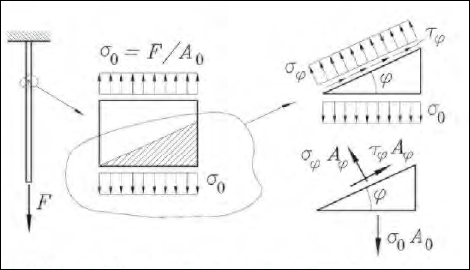
\includegraphics[width=0.8\textwidth]{einachsspann}
\caption{Einachsiger Spannungszustand am Zugstab}
\label{fig:einachsspann} 
\end{figure}
Bei Belastung eines Bauteils in nur einer Richtung liegt der sogenannte einachsige Spannungszustand vor. Wenn man an dem Zugstab \fref{fig:einachsspann} einen Schnitt nicht senkrecht zur Richtung von $ \sigma_0 $ betrachtet erkennt man, dass dort auch Schubspannungen im Bauteil vorhanden sind. Um einen Gleichgewichtszustand in horizontaler Richtung an dem herausgeschnittenen Keil herzustellen ist es nötig das in der schrägen Schnittfläche $ A_{\varphi} $ außer der Nomalspannung $ \sigma_{\varphi} $ zusätzlich die Schubspannung $ \tau_{\varphi} $ vorhanden ist. Durch Multiplikation der Spannungen in den Schnittflächen $ A_0 $ und $ A_{\varphi} $ mit den entsprechenden Flächen erhält man die Kräfte $ \sigma_0 \A_0 $ und $ \sigma_{\varphi} A_{\varphi} $. Es können nun fogende Gleichgewichtsbedingungen aufgestellt werden \begin{equation}
\sigma_{\varphi}A_{\varphi} - \sigma_0 A_0\cos{\varphi} = 0  
\end{equation}
\begin{equation}
\tau_{\varphi}A_{\varphi} - \sigma_0A_0\sin{\varphi} = 0
\end{equation} Durch Einsetzten von $ A_0 = A_{\varphi}\cos{\varphi}$ erhält man die Gleichungen für die Spannungen in einem beliebigen Schnitt bei dem einachsigen Spannungszustand
\begin{equation}
\sigma_{\varphi} = \sigma_0\cos^2{\varphi}
\end{equation}
\begin{equation}
\tau_{\varphi} = \frac{1}{2} \sigma_0\sin{2\varphi}
\end{equation}
Aus diesen Gleichungen ist zu erkennen das die Normalspannung am größten bei $ \varphi = 0 $ ist, weil in dem Schnitt keine Schubspannung vorhanden ist. Deshalb wird $ \sigma_0 $ in diesem Fall als \emph{Hauptspannung} bezeichnet. Die maximale Schubspannung ergibt sich bei $ \varphi = 45^{\circ} $ sie wird als \emph{Hauptschubspannung} ($ \tau_{\text{max}} = \frac{1}{2}\sigma_0 $ ) bezeichnet.\footcite[Vgl.][388]{dd}



  
\subsubsection{Spannungsvektor und Spannungstensor}
Zum besseren Verständnis was für Kräfte und Spannungsverhältnisse bei Umformvorgängen im Material vorherrschen ist es sinnvoll sie an infinitesimal kleinen Volumenelementen zu modellieren. Dazu stellt man sich einen Körper unter Belastung der Einzelkräfte $ F_i $ und der Flächenlasten $ p $ \ vor ( siehe \fref{fig:normalvektor}) \footcite [Vgl.][43]{tmr}. Äußere Belastungen verursachen grundsätzlich auch innere Kräfte in einem Bauteil. Betrachtet man den Schnitt s--s \begin{figure}
  \centering
  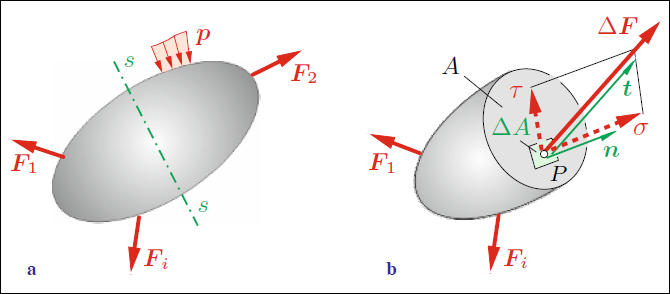
\includegraphics[width=0.8\textwidth]{normalvektor}
  \caption{Spannungsvektor an beliebigen Körper}
  \label{fig:normalvektor}
  \end{figure} erkennt man das die inneren Kräfte sowie Spannungen über die ganze Schnittfläche $ A $ verteilt sind. Spannung sind über die Schnittfläche veränderlich deshalb  wird ein beliebiger Punkt $ P $ der Schnittfläche definiert. Die Schnittkraft $ \Delta F $  wirkt auf ein Flächenelement $ \Delta A $ (in dem $ P $ enthalten ist). Es wirkt eine gleich große entgegengesetzte Kraft auf die gegenüberliegende Schnittfläche (actio gleich reactio). Der Quotient $ \frac{\Delta F}{\Delta A} $ (Kraft auf die Fläche bezogen) definiert die mittlere Spannung für das Flächenelement. Wenn man nun bei der Beziehung $ \frac{\Delta F}{\Delta A} $ den Differentialquotienten bildet in dem $ \Delt A \rightarrow 0 $ gegen Null läuft  resultiert daraus die Formel für den \emph{Spannungsvektor }$ t $ \begin{equation}
   t = \lim \limits_{\Delta A \to 0} \frac{\Delta F}{\Delta A} = \frac{\text{d}F}{\text{d}A}  
   \end{equation}
Der Spannungsvektor lässt sich in eine Komponente normal zur Schnittfläche ( \emph{Normalspannung} $ \sigma $) und eine Komponente in der Schnittfläche (tangentiale \emph{Schubspannung} $ \tau $) zerlegen. Es existiert eine Abhängigkeit des Spannungsvektors $ t $ von der Lage des Punktes $ P $ in der Schnittfläche. Also eine Ortsabhängigkeit. Kann der Spannungsvektor $ t $ für alle Punkt von A angegeben werden, so ist die Spannungsverteilung in der Schnittfläche bekannt. Dennoch wird durch $ t $ der Spannungszustand in einem Punkt $ P $ nicht vollständig definiert. Werden durch $ P $ Schnitte in verschiedene Richtungen gelegt, so wirken entsprechend der unterschiedlichen Orientierung der Flächenelemente auch unterschiedliche Schnittkräfte. Es liegt demzufolge auch eine Schnittrichtungsabhängigkeit der Spannungen vor. Die Schnittrichtung wird von dem Normalenvektor $ n $ charakterisiert. Der Spannungszustand in einem Punkt $ P $ wird durch drei Spannungsvektoren in drei senkrecht aufeinander stehenden Schnittflächen festgelegt. Zu Darstellungszwecken fallen die drei Schnittflächen in dieser Modellierung mit den Koordinatenebenen eines kartesischen Koordinatensystems zusammen.

Um sie prägnant darzustellen, visualisiert man sie als Seitenflächen eines infinitesimalen Quaders mit den Kantenlängen d$ x $, d$ y $ und d$ z $ in der Umgebung von $ P $\begin{figure}
  \centering
  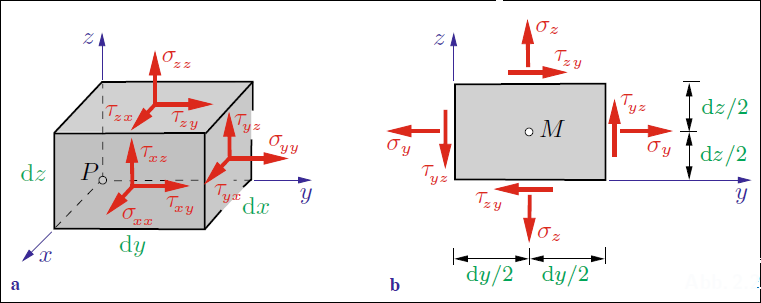
\includegraphics[width=0.8\textwidth]{tensor}
  \caption{Spannungen und Kräfte am Infinitesimalelement}
  \label{fig:tensor}
  \end{figure}( siehe \fref{fig:tensor})\footcite[Vgl.][44]{tmr} . Ein Spannungsvektor wirkt hier je Fläche, der in seine Komponenten senkrecht zur Schnittfläche (daraus folgt Normalspannung) und in der Schnittfläche (daraus folgt Schubspannung) zerlegt wird. Zusätzlich werden die Schubspannungen noch in die Komponenten der Richtung der Koordinatenachsen zerlegt. Es werden Doppelindizes zur Kennzeichnung der jeweiligen Komponenten benutzt(siehe \fref{fig:tensor}). 
Der erste Index kennzeichnet die Richtung der Flächennormalen, wohingegen der zweite Index die Richtung der Spannungskomponenten bezeichnet. Zum Beispiel deklariert $ \tau_{yx} $ die Schubspannung einer Ebene, deren Normale in $y$ - Richtung weist. Die Spannung zeigt hier in die $ x $ - Richtung (siehe \fref{fig:tensor}). Es ist sinnvoll und vermeidet Verwechselungen bei den Normalspannungen die Schreibweise zu simplifizieren. Spannung und Flächennormale besitzen in diesem Fall die gleiche Richtung. Daraus ergibt sich eine Übereinstimmung der beiden Indizes und es ist hinreichend nur einen Index anzugeben. Es ist also völlig ausreichend  folgende Angaben zu machen: $ \sigma_{xx} = \sigma_{x} $, $ \sigma_{yy} = \sigma_y $, $ \sigma_{zz} = \sigma_z $.

Der Spannungsvektor für die Schnittfläche, deren Normale in $ y $ - Richtung zeigt wir mit den oben angeführten Konventionen zu folgender Formel:
\begin{equation}
t = \tau_{yx}e_x + \sigma_ye_y + \tau_{yz}e_z
\end{equation}

Analog zu den Schnittgrößen existiert für die Spannungen eine \emph{Vorzeichenkonvention}:

"`\emph{Positive} Spannungen zeigen an einem positiven (negativen) Schnittufer in die positive (negative) Koordinatenrichtung."'\footcite[45]{tmr}

Infolgedessen beanspruchen positive (negative) Normalspannungen den infinitesimalen Quader auf Zug (Druck). Nach Zerlegung der Spannungsvektoren in ihre Komponenten erhält man drei Normalspannungen ($ \sigma_x$, $ \sigma_y $, $ \sigma_z $) und sechs Schubspannungen ( $ \tau_{xy}, \tau_{xz}, \tau_{yx}, \tau_{yz}, \tau_{zx}, \tau_{zy} $), die jedoch nicht alle unabhängig voneinander sind. Um das zu beweisen wird das Momentengleichgewicht um eine zur $x$- Achse parallele Achse durch den Mittelpunkt des Quaders (siehe \fref{fig:tensor})aufgestellt. Unter der Berücksichtigung das Gleichgewichtsaussagen nur für Kräfte gelten, werden die Spannungen mit den zugeordneten Flächenelementen multipliziert.
\begin{equation}
\overset{\curvearrowleft}{M}: 2\,\frac{\text{d}y}{2}\,(\tau_{yz}\,\text{d}x\,\text{d}z) - 2\,\frac{\text{d}z}{2}\,(\tau_{zy}\, \text{d}x\,\text{d}y)\,= 0 \Rightarrow\,\tau_{yz} = \tau_{zy}
\end{equation} Analog dazu gilt für die anderen Achsen: \begin{equation}
\tau_{xy}=\tau_{yx},\quad\tau_{xz}=\tau_{zx},\quad\tau_{yz}=\tau_{xy}
\end{equation}

Aus dem folgt:

"`Schubspannungen in zwei senkrecht aufeinander stehenden Schnitten (z.B. $\tau_{xy}$ und $\tau_{zy}$) sind gleich."'\footcite[46]{tmr}

Sie werden als einander \emph{zugeordnete Schubspannungen} bezeichnet. Aufgrund der Tatsache das sie gleiche Vorzeichen besitzen, deuten sie entweder auf die gemeinsame Quaderkante oder sie sind beide von ihr abgewandt. Wie aus den oben angeführten Identitäten zu erkennen ist, existieren lediglich sechs unabhängige Spannungen. Die Komponenten der jeweiligen Spannungsvektoren lassen sich in einer Matrix anordnen:
\begin{equation}
\sigma = \begin{pmatrix}
\sigma_x & \tau_{xy} & \tau_{xz}\\
\tau_{yx} & \sigma_y & \tau_{yz}\\
\tau_{zx} & \tau_{zy} & \sigma_z
\end{pmatrix} = \begin{pmatrix}
\sigma_x & \tau_{xy} & \tau_{xz}\\
\tau_{xy} & \sigma_y & \tau_{yz}\\
\tau_{xz} & \tau_{yz} & \sigma_z
\end{pmatrix}
\end{equation}

Die Normalspannungen bilden die Hauptdiagonale. Alle anderen Elemente sind Schubspannungen. Die Matrix ist symmetrisch und stellt den \emph{Spannungstensor} dar. Er wird mit der Größe $ \sigma $ bezeichnet. Der \emph{Spannungszustand} wird durch den \emph{Spannungstensor} (Spannungsvektoren für drei aufeinander stehende Schnitte) eindeutig in einem Punkt festgelegt.\footcite[Vgl.][43-46]{tmr}
\subsubsection{Festigkeitshypothesen}
In der Praxis unterliegen Bauteile nahezu immer einem mehrachsigen Spannungszustand. Zulässige Spannungen $ \sigma_{zul} $ für Bauteile und Werkstoffe werden aber meistens mit dem einachsigen Zugversuch in Laboren festgelegt. Um nun die realen Spannungsverhältnisse im Bauteil mit den Laborwerten vergleichbar zu machen bedient man sich bestimmter Festigkeitshypothesen, die die Hauptspannungen berücksichtigen um sie mit den theoretischen Mindestzugfestigkeiten gegenüberzustellen. Es wird also zuerst unter zu Hilfenahme einer Spannungshypothese eine Vergleichsspannung $ \sigma_V $ errechnet  und diese dann mit $ \sigma_{zul} $ verglichen. Idealisiert würde solch eine Vergleichsspannung alle wirkenden Veränderungen und Spannungen sowie Veränderungen des Materialverhaltens (z.B. Fließen, Bruch) bei gleichen Werten auslösen wie im einachsigen Spannungszustand bei dem modellierten Zugversuch. Bei der Gegenüberstellung der beiden Spannungen gilt dann $ \sigma_V \leq \sigma_{zul} $. Es wurden im laufe der Jahre zahlreiche solcher Spannungshypothesen hergeleitet.\footcite[Vgl.][399]{dd} Hier sollen nur die geläufigsten, nämlich die Spannungshypothesen von  \emph{Tresca} und \emph{von Mises} kurz vorgestellt werden.

Die \emph{Schubspannungshypothese} nach Tresca geht davon aus, dass die Materialbeanspruchung durch die maximale Schubspannung zu charakterisieren ist. Für den dreidimensionalen Spannungszustand gilt die Formel \begin{equation} \sigma_V = \sqrt{(\sigma_x - \sigma_y )^2 + 4\tau^2_{xy}} \end{equation}. Bei der \emph{Hypothese der Gestaltänderungsenergie} nach von Mieses wird davon ausgegangen, dass die zur Änderung der Gestalt benötigte Energie zu Vergleichszwecken herangezogen wird. Für den räumlichen Spannungszustand wird folgernder Term gegeben: \begin{equation} \sigma_V = \sqrt{\sigma^2_x + \sigma^2_y - \sigma_x\sigma_y + 3\tau^2_{xy}} \end{equation} 
Die Hypothese der Gestaltänderungsenergie ist besonders bei zähen Werkstoffen aussagekräftiger und präziser als die Schubspannungshypothese.\footcite[Vgl.][84]{tmr}




























